\documentclass[11pt,a4paper]{article}
% Shared preamble for the three Phase 2 deliverables
\usepackage[utf8]{inputenc}
\usepackage[T1]{fontenc}
\usepackage{lmodern}
\usepackage[margin=2.3cm]{geometry}
\usepackage{graphicx}
\usepackage{xcolor}
\usepackage{booktabs}
\usepackage{enumitem}
\usepackage{titlesec}
\usepackage{fancyhdr}
\usepackage{tcolorbox}
\usepackage{float}
\usepackage{caption}
\usepackage{parskip}
\usepackage{listings}
\usepackage{array}
\usepackage{hyperref}

\definecolor{primary}{RGB}{44,62,80}
\definecolor{accent}{RGB}{52,152,219}
\definecolor{insightbg}{RGB}{235,245,255}
\definecolor{bodytext}{RGB}{50,50,50}
\definecolor{kw}{RGB}{0,92,170}
\definecolor{cm}{RGB}{110,110,110}
\definecolor{st}{RGB}{163,21,21}
\definecolor{codebg}{RGB}{248,249,251}

\hypersetup{colorlinks=true, linkcolor=accent, urlcolor=accent,
  pdfauthor={Saanvi Grover, Aditya Sharma}}

\titleformat{\section}{\Large\bfseries\color{primary}}{}{0em}{}[\color{accent}\titlerule]
\titleformat{\subsection}{\large\bfseries\color{primary}}{}{0em}{}
\titleformat{\subsubsection}{\normalsize\bfseries\color{primary}}{}{0em}{}

\pagestyle{fancy}
\fancyhf{}
\fancyfoot[C]{\thepage}
\renewcommand{\headrulewidth}{0pt}

\lstdefinelanguage{SQLplus}[]{SQL}{
  morekeywords={WITH, OVER, PARTITION, RANK, NTILE, PERCENT_RANK, COALESCE, ROUND,
                CROSS, RETURNING, WINDOW, ROWS, PRECEDING, FOLLOWING, CURRENT, UNBOUNDED},
  sensitive=false
}
\lstset{
  language=SQLplus,
  basicstyle=\ttfamily\footnotesize\color{bodytext},
  keywordstyle=\color{kw}\bfseries,
  commentstyle=\color{cm}\itshape,
  stringstyle=\color{st},
  backgroundcolor=\color{codebg},
  frame=single, rulecolor=\color{accent}, framerule=0.4pt,
  numbers=left, numberstyle=\tiny\color{cm}, numbersep=8pt,
  breaklines=true, showstringspaces=false, tabsize=4,
  xleftmargin=1.6em, aboveskip=6pt, belowskip=6pt, columns=fullflexible, keepspaces=true
}

\newtcolorbox{insightbox}[1][KEY INSIGHT]{
  colback=insightbg, colframe=accent, boxrule=0.5pt, arc=2pt,
  left=8pt, right=8pt, top=6pt, bottom=6pt,
  fonttitle=\bfseries\color{accent}\small, title=#1
}

\newcommand{\entropytitle}[2]{%
\begin{titlepage}
\centering
\vspace*{3.5cm}
{\Huge\bfseries\color{primary} #1\par}
\vspace{0.6cm}
{\Large\color{gray} #2\par}
\vspace{1.2cm}
{\color{accent}\rule{8cm}{1pt}\par}
\vspace{1.2cm}
{\large\color{gray} Round 1, Phase 2: Analytical Core\par}
\vspace{1.5cm}
{\large
\begin{tabular}{rl}
\textbf{Competition:} & Data Vortex $|$ AARUUSH'26 \\
\textbf{Theme:} & Rebuilding the Social Engine \\
\textbf{Team:} & Entropy \\
\textbf{Members:} & Saanvi Grover \& Aditya Sharma \\[0.4cm]
\textbf{Questions:} & E3 $\cdot$ M4 $\cdot$ H4 \\
\textbf{Database:} & SQLite (\texttt{Entropy\_social\_engine.db}) \\
\end{tabular}
\par}
\vfill
\end{titlepage}
}

\hypersetup{pdftitle={Phase 2 Insight Report -- Team Entropy}}

\begin{document}
\color{bodytext}
\entropytitle{Phase 2 Insight Report}{Key insights and findings from E3, M4 and H4}

\section{Executive Summary}

Three questions, three levels, one consistent answer: in the Social Engine dataset, \textbf{engagement is not explained by platform, by audience size, or by any user attribute}. Each query was designed to test one of these levers against a built-in benchmark, and each time the ``winner'' turned out to be within noise of the field.

\begin{table}[H]
\centering\small
\begin{tabular}{@{}lp{4.6cm}p{6.6cm}@{}}
\toprule
\textbf{Question} & \textbf{Literal answer} & \textbf{What it actually means} \\
\midrule
E3 & Instagram: 4,040.0 avg total engagement & All five platforms sit within 2.2\% of each other (Kruskal--Wallis $p = 0.56$). Platform choice is irrelevant. \\
M4 & Instagram: 4,145.2 for users with $\geq$ 30k followers & The high-follower cohort tracks the all-user baseline platform by platform (Mann--Whitney $p = 0.98$). A large audience buys nothing. \\
H4 & 16 users with $<$ 5k followers in the top 10\% & Chance alone predicts 13.1 (binomial $p = 0.39$). They are there because they post 61\% more often, not because their posts perform better. \\
\bottomrule
\end{tabular}
\end{table}

\begin{insightbox}[HEADLINE]
The only lever that moves \emph{total} engagement in this dataset is volume: post count explains user totals almost completely (Spearman $\rho = 0.89$), while follower count explains nothing ($\rho = -0.03$). Any ``high-performing'' or ``suspicious'' account list built on totals is really a list of frequent posters.
\end{insightbox}

\section{E3 -- Does Platform Choice Matter?}

\begin{figure}[H]\centering
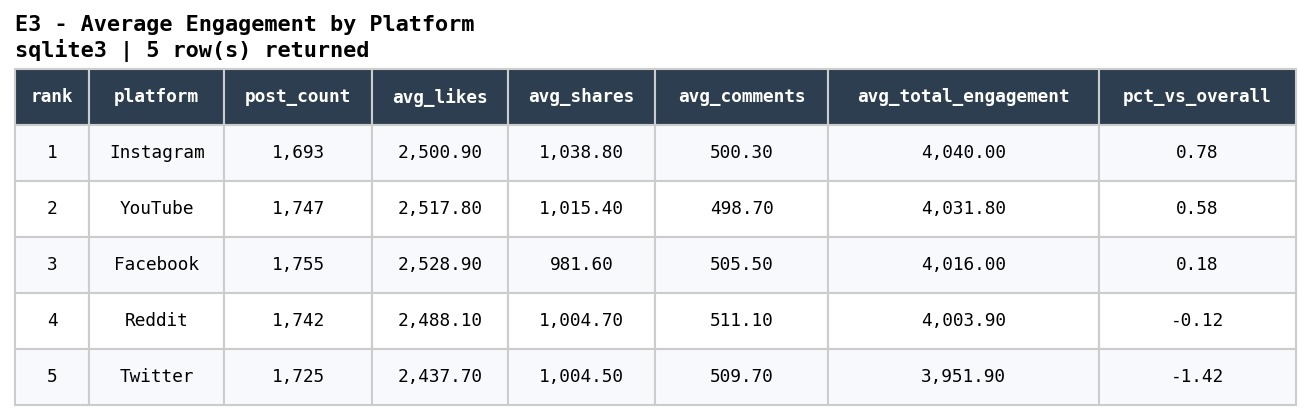
\includegraphics[width=0.9\textwidth]{images/Entropy_E3_output.jpeg}
\caption{E3 query output (5 rows).}
\end{figure}

\subsection{Findings}
\begin{itemize}[leftmargin=*]
  \item Instagram leads with an average total engagement of 4,040.0 per post; Twitter is last at 3,951.9. The gap between first and last is 88 points, or \textbf{2.2\% of the mean}.
  \item The three components are flat too: average likes range 2,438--2,529, shares 982--1,039, comments 499--511 across platforms.
  \item Each platform received 1,693--1,755 posts with valid data, so no ranking is driven by a small sample.
\end{itemize}

\begin{figure}[H]\centering
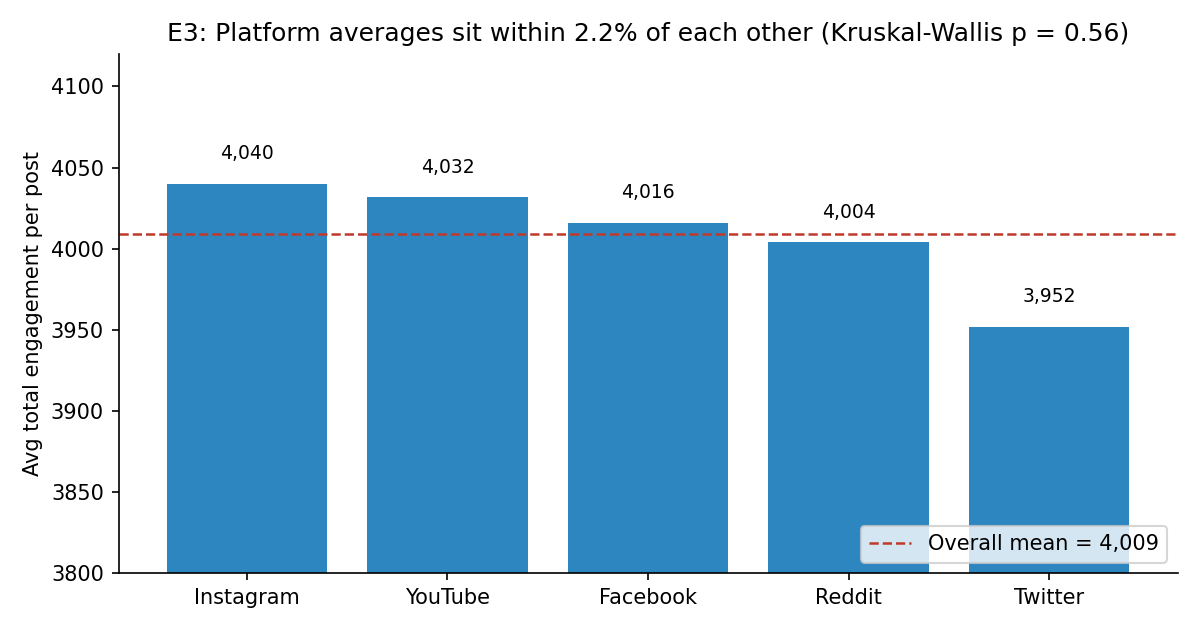
\includegraphics[width=0.8\textwidth]{images/Entropy_E3_insight_chart.png}
\caption{Platform averages against the overall mean. The y-axis is truncated to make the differences visible at all.}
\end{figure}

\begin{insightbox}
Real platforms differ 2--3$\times$ in engagement; here they differ by 2\%. Instagram is ``highest'' in the same sense that one coin landed heads slightly more often in 1,700 flips. The correct business reading is that content should be distributed by audience fit, not by expected engagement.
\end{insightbox}

\section{M4 -- Do Large Audiences Behave Differently?}

\begin{figure}[H]\centering
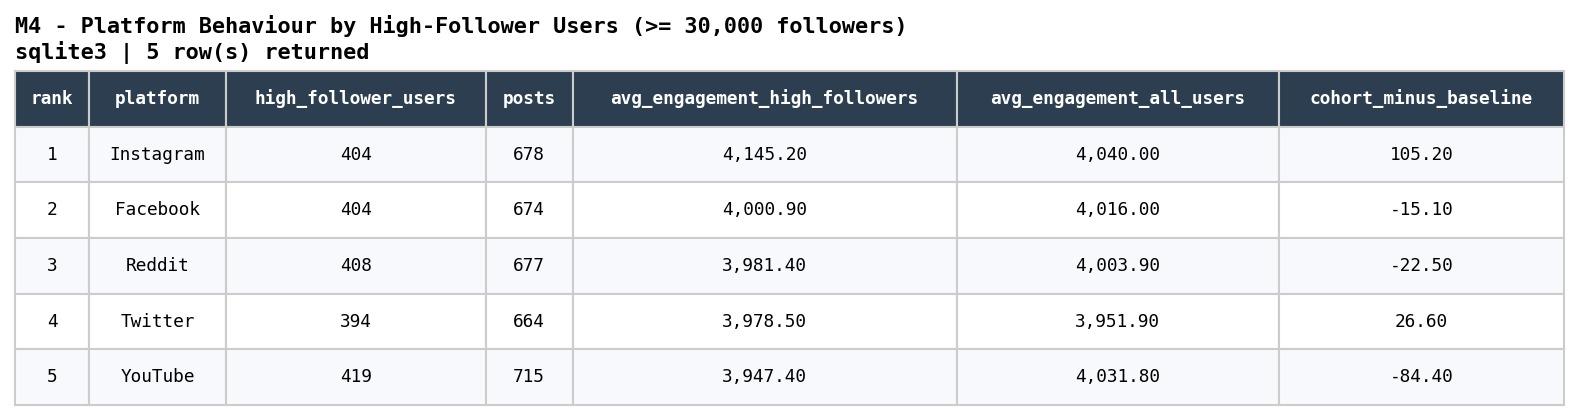
\includegraphics[width=0.95\textwidth]{images/Entropy_M4_output.jpeg}
\caption{M4 query output (5 rows) with the all-user baseline for each platform.}
\end{figure}

\subsection{Findings}
\begin{itemize}[leftmargin=*]
  \item 594 users (39.6\%) have at least 30,000 followers; together they contribute 3,408 posts with valid data.
  \item Their best platform is again Instagram at 4,145.2 per post, $+105$ above Instagram's all-user average. Their worst is YouTube at 3,947.4, $-84$ below YouTube's baseline.
  \item Three of five platforms show the cohort \emph{below} baseline. The largest deviation in either direction is about 2.6\%.
  \item Within the cohort, platform differences are not significant (Kruskal--Wallis $p = 0.18$), and the cohort's posts are statistically identical to everyone else's (Mann--Whitney $p = 0.98$).
\end{itemize}

\begin{figure}[H]\centering
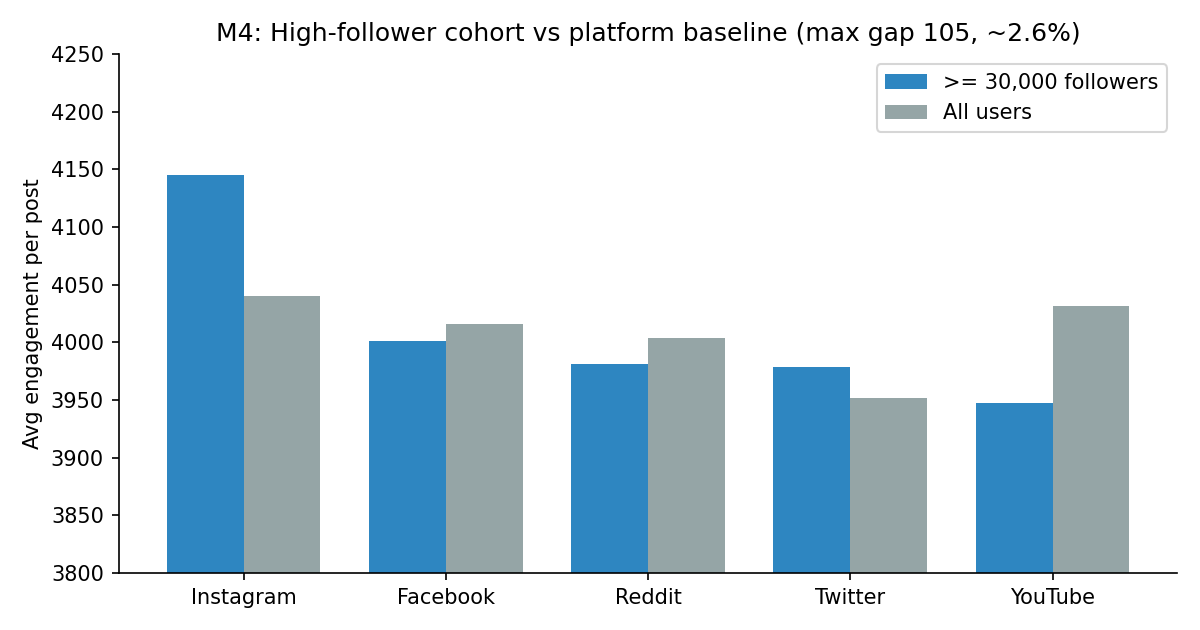
\includegraphics[width=0.8\textwidth]{images/Entropy_M4_insight_chart.png}
\caption{High-follower cohort vs.\ baseline by platform.}
\end{figure}

\begin{insightbox}
If follower count mattered, the 30k+ cohort would sit above every baseline bar. Instead it straddles them. Whatever generated this data assigned engagement independently of the author, so an influencer strategy (paying for reach) would not change results here. The Instagram ``preference'' is a 2.6\% ripple, not a behaviour.
\end{insightbox}

\section{H4 -- Are Low-Follower Top Performers Anomalous?}

\begin{figure}[H]\centering
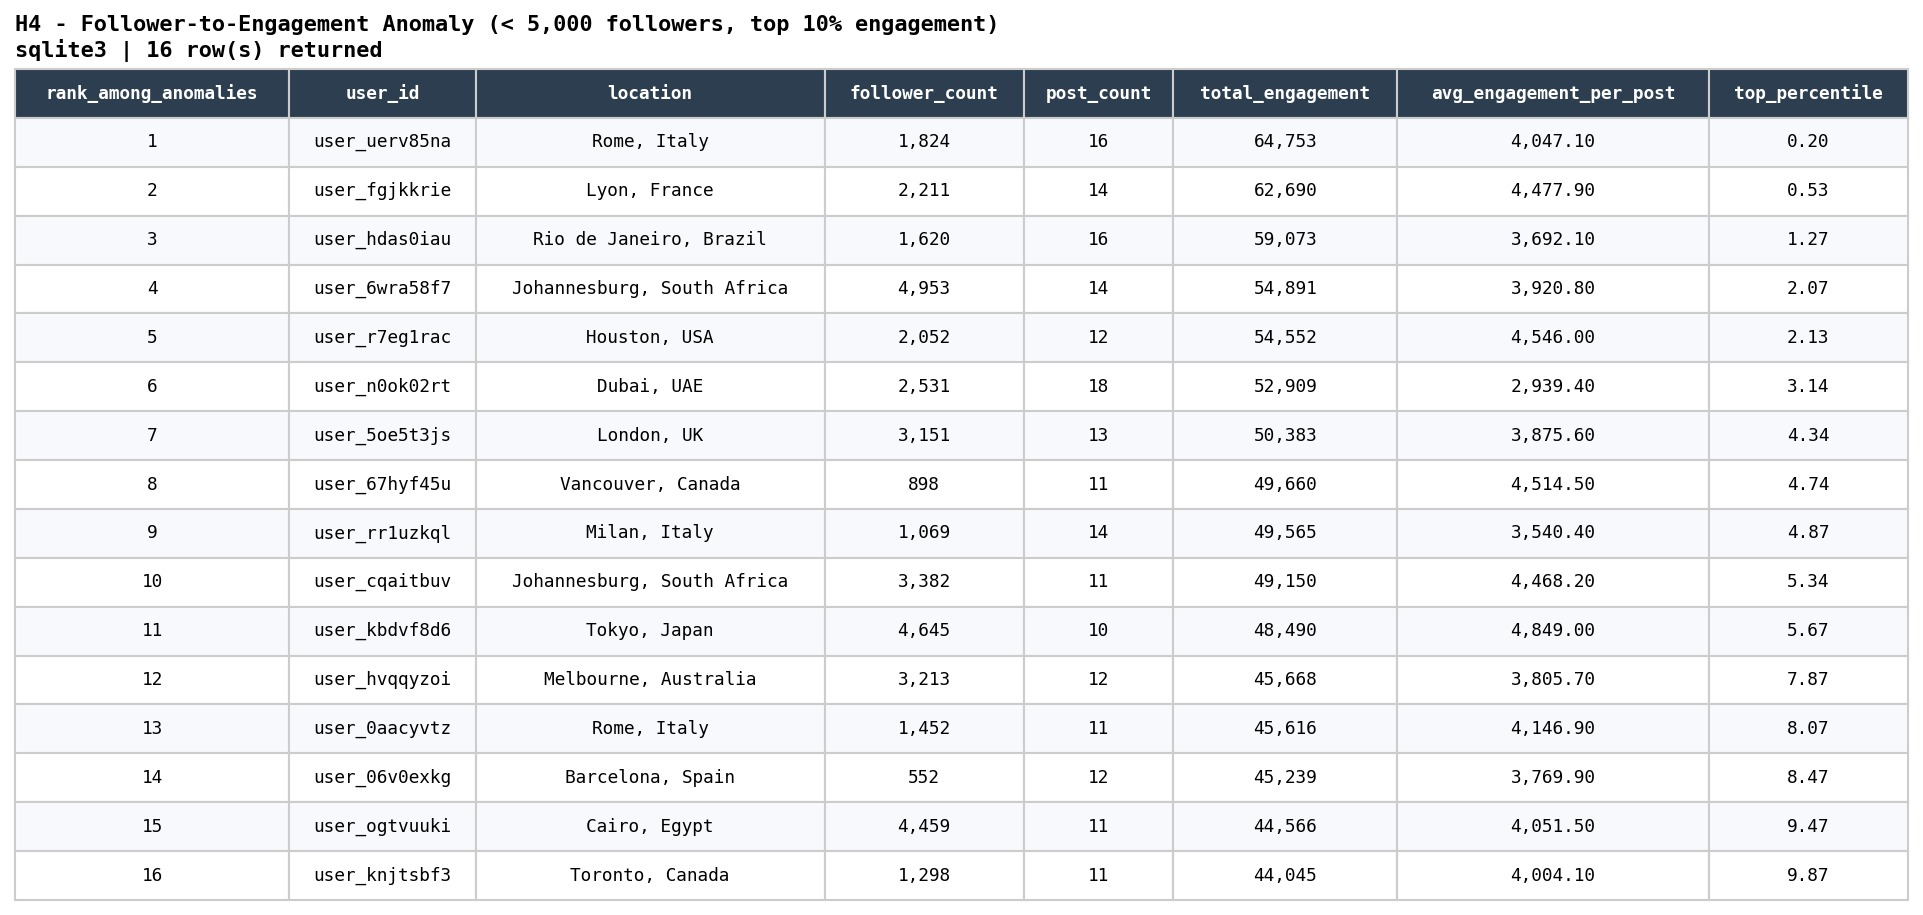
\includegraphics[width=\textwidth]{images/Entropy_H4_output.jpeg}
\caption{H4 query output: 16 users with fewer than 5,000 followers inside the top engagement decile.}
\end{figure}

\subsection{Findings}
\begin{itemize}[leftmargin=*]
  \item The top 10\% of users by total engagement is 150 users, with a threshold of 43,948. Sixteen of them have fewer than 5,000 followers, led by \texttt{user\_uerv85na} (Rome; 1,824 followers; 64,753 total engagement, the top 0.2\% of all users).
  \item \textbf{Expected vs.\ observed.} 131 users (8.73\%) have $<$ 5,000 followers. If followers and engagement are independent, $150 \times 0.0873 = 13.1$ of them should land in the top decile. Observing 16 has a binomial probability of 0.39; the excess is well inside chance.
  \item \textbf{What puts them there.} The 16 average \textbf{12.9 posts each} versus 8.0 for the population (and 12.75 for the whole top decile). Their engagement \emph{per post} is 2,939--4,849, centred on $\sim$4,040, essentially the platform-wide mean from E3.
  \item Across all users, post count vs.\ total engagement gives $\rho = 0.89$; follower count vs.\ total engagement gives $\rho = -0.03$ ($p = 0.30$); follower count vs.\ per-post average gives $\rho = -0.03$ ($p = 0.34$).
\end{itemize}

\begin{figure}[H]\centering
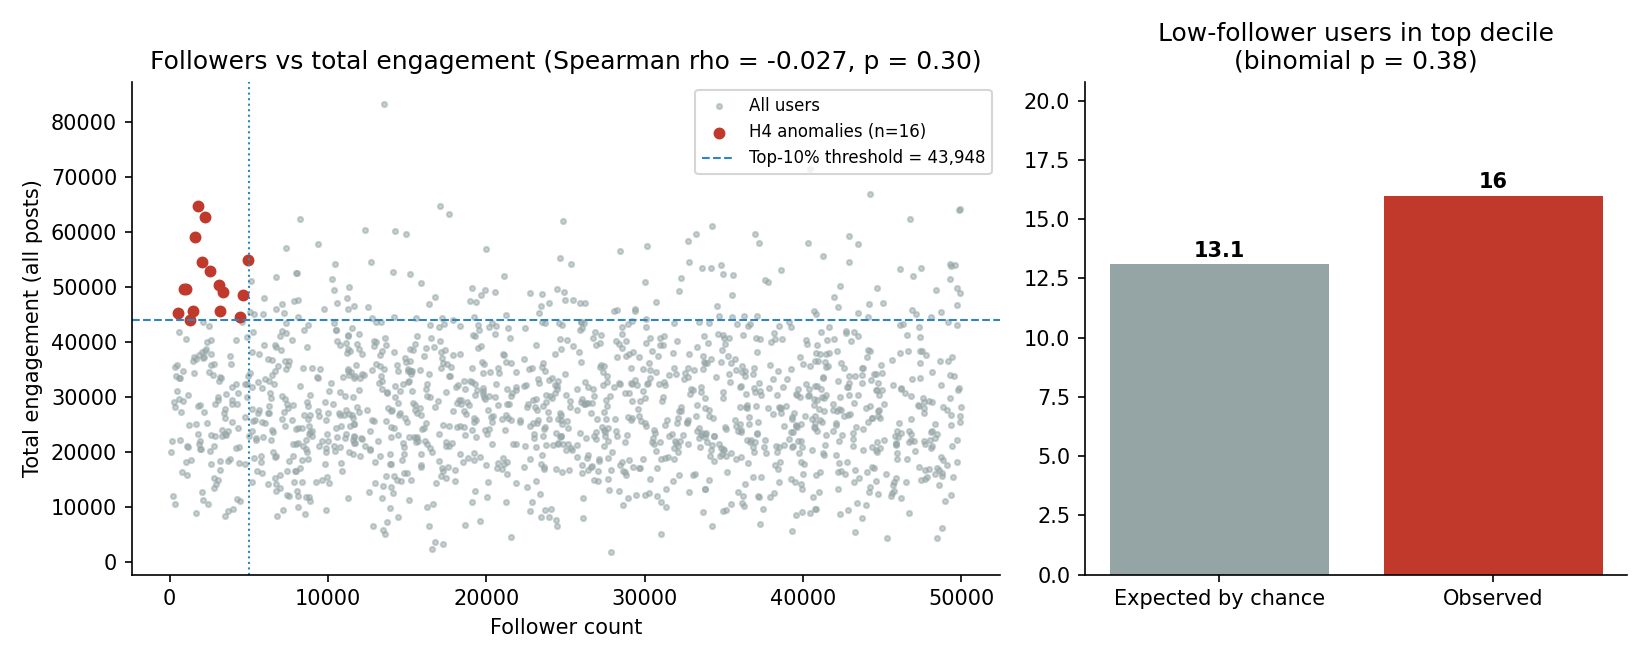
\includegraphics[width=\textwidth]{images/Entropy_H4_insight_chart.png}
\caption{Left: the 16 anomalies (red) occupy the low-follower/high-total corner, but the cloud is flat in the follower dimension. Right: observed vs.\ expected count under independence.}
\end{figure}

\begin{figure}[H]\centering
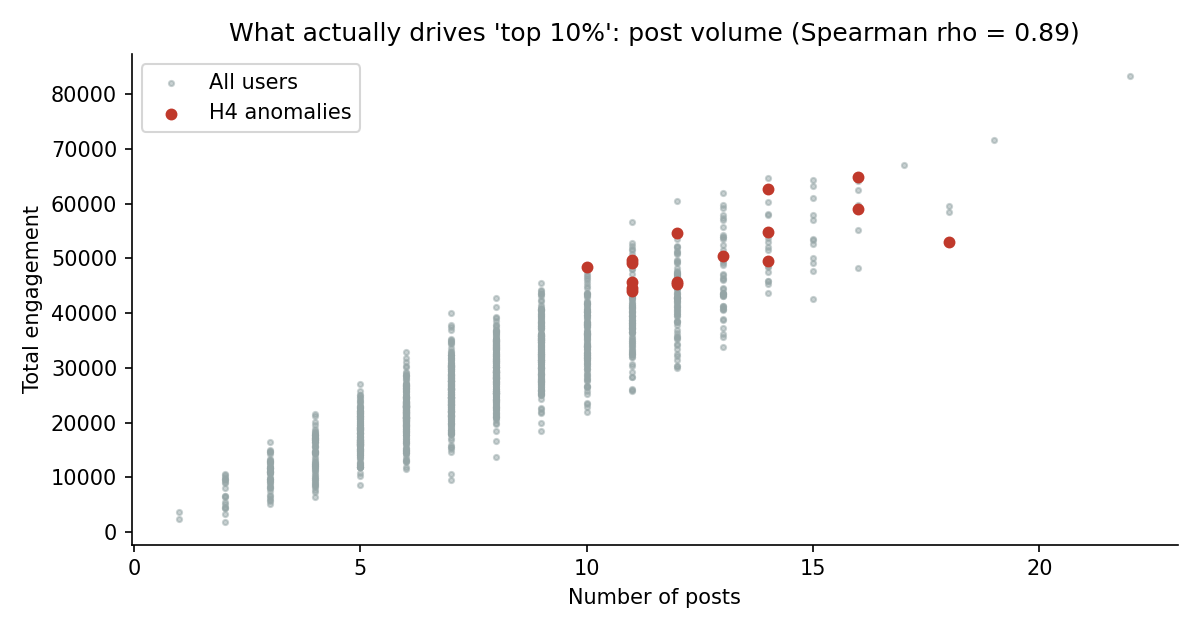
\includegraphics[width=0.8\textwidth]{images/Entropy_H4_post_volume_chart.png}
\caption{Total engagement is almost a linear function of post count; the anomalies are simply the most prolific low-follower users.}
\end{figure}

\begin{insightbox}
The brief suggests these users ``may represent unusually high performing or suspicious accounts''. The data says neither: they perform at the population average and appear at the frequency independence predicts. A fraud or talent team acting on this list would be chasing sampling noise. A meaningful version of this question would rank on \emph{per-post} engagement, which removes the volume effect entirely.
\end{insightbox}

\section{Cross-Question Synthesis}

\begin{table}[H]
\centering\small
\begin{tabular}{@{}lccl@{}}
\toprule
\textbf{Lever tested} & \textbf{Largest effect found} & \textbf{Significance} & \textbf{Verdict} \\
\midrule
Platform (E3) & 2.2\% spread & $p = 0.56$ & No effect \\
Audience size $\times$ platform (M4) & 2.6\% vs.\ baseline & $p = 0.18$ / $0.98$ & No effect \\
Audience size vs.\ total engagement (H4) & $\rho = -0.03$ & $p = 0.30$ & No effect \\
Post volume vs.\ total engagement (H4) & $\rho = 0.89$ & $p < 10^{-100}$ & Dominant driver \\
\bottomrule
\end{tabular}
\caption{Every user-facing lever is flat; only volume moves totals.}
\end{table}

These results are consistent with the Phase 1 EDA, where 5 of 6 hypothesis tests returned $p > 0.05$ and coefficient-of-variation analysis showed most dimensions below 10\% variation. Phase 2 sharpens that picture in one respect: the dataset does contain a real, strong relationship (posts $\rightarrow$ totals), so ``no signal anywhere'' would be the wrong conclusion. The signal is just not in the places the questions point to.

\section{Recommendations}

\begin{enumerate}[leftmargin=*]
  \item \textbf{Normalise before ranking.} Any leaderboard, anomaly list or ``top user'' report on this data must use per-post engagement, otherwise it measures activity, not quality.
  \item \textbf{Do not segment by platform or follower tier.} Both segmentations return differences of 2--3\%, below any practical threshold; resources spent on platform-specific or influencer-specific strategy would be wasted.
  \item \textbf{Treat the multi-platform effect as the lead for Round 3.} It was the only significant lever in Phase 1 ($\sim$15\% higher engagement) and remains untouched by the three questions here.
  \item \textbf{Keep the NULL policy explicit.} The 15\% MCAR corruption is harmless for averages if rows are excluded consistently, and for sums if treated as zero; mixing the two silently biases results by up to 15\%.
\end{enumerate}

\end{document}
